\chapter{Data-Oblivious Sorting Algorithms}
\label{ch:algorithms}

Throughout this thesis, several data-oblivious sorting algorithms will be discussed, and their properties relating to efficiency and optimization techniques will be studied. Before we can continue on to this work, we must however ensure that we have established the structure of these algorithms, and most of this chapter will devote itself to brief descriptions of the individual algorithms that form the basis of any further work being done.

Let us begin by immediately describing these algorithms. 

\section{Randomized Shellsort}

Randomized Shellsort~\citeA{RandShellSort} is a randomized data-oblivious sorting algorithm notable for its ability to sort data with very high probability, using only $\Theta(n \log n)$ comparisons.

The algorithm itself is fairly simplistic, consisting entirely of applications of a special region comparison function, whose method of operation will be described shortly. This can then optionally be followed by clean-up phase entirely constructed from already known data-oblivious sorting algorithms.

It is especially important to note that the size and location of regions being compared will be entirely dependent on the size of the data, and that matchings between elements is determined randomly with no knowledge of the input.

The analysis showing the low failure rate of the algorithm is unfortunately rather lengthy, and somewhat complex, but can be found in~\citeA{RandShellSort}.

\subsection{Region Comparison}
\label{sec:RegionCompare}

The comparison between regions is done by computing a random matching between elements of the two regions, and performing a \texttt{Compare-Exchange} operation between each pair of matched indices.
This procedure will be repeated $c$ times to perform a full comparison of regions.~\citeA{RandShellSort} shows that when $c \geq 4$ the full region comparison will have properties closely related to those of \textepsilon -halvers.

The pseudo-code for the region comparison is shown in Algorithm~\ref{RegionCompare}.

For a graphical representation of the region comparison, see Figure~\ref{fig:CompareExchange}.


\begin{algorithm}
\caption{Region Compare}\label{RegionCompare}
\begin{algorithmic}[1]
	\Statex $A$: Array input of \texttt{Compare-Exchange} compatible elements
	\Statex $i$: Index of first region
	\Statex $j$: Index of second region
	\Statex $size$: Size of regions to compare
\Procedure{RegionCompare}{$A, i, j, size$}
\For{$1 \dots c$}
	\Comment $c$ is a predetermined constant
	\State $matching \gets \mathtt{shuffle}([0 \dots size-1])$
	\For{$k = 0 \dots size-1$}
		\State $\mathtt{Compare\mbox{-}Exchange}(A, i + k, j + matching[k])$
	\EndFor
\EndFor
\EndProcedure
\end{algorithmic}
\end{algorithm}

\begin{figure}
\center
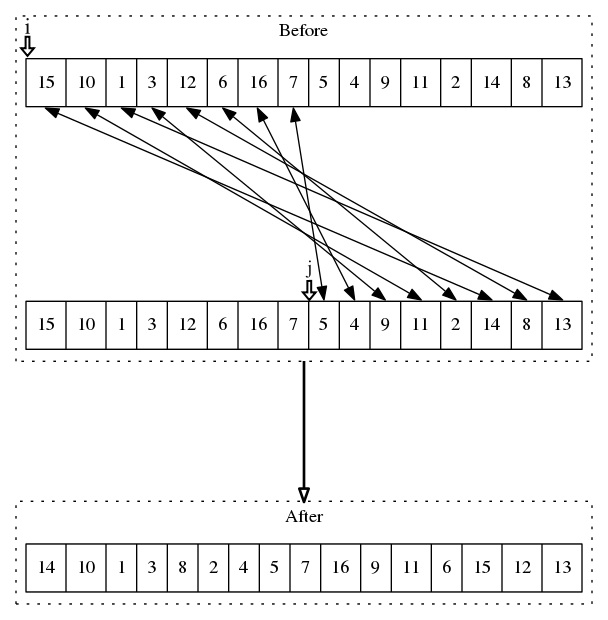
\includegraphics[width=\textwidth]{Graphics/regcmp.png}
\caption{Region Compare with $c=1$ of size 8 on 16 elements of data. $i$ and $j$ are the first and last halves of the shown arrays respectively. Note that the \emph{Before} region shows the matching with the same array.}
\label{fig:CompareExchange}
\end{figure}

\subsection{The Main Algorithm}

Having constructed the region comparison operation, we move on to the main algorithm.

The important part of Randomized Shellsort consist of applying the region comparison on the input data in ever decreasing region sizes, starting at $n/2$, and halving in size until they reach $1$. Note that there will be only $\log(n)$ such region sizes, and that $n$ is assumed to be a non-trivial power of 2.

For each region size, six different runs through the data are performed. These runs fall into two distinct groups, a \emph{shaker} phase and a \emph{brick} phase.

In the \emph{shaker} phase we run through the regions, comparing them with the next region in ascending order, and then do the same for descending order. This resembles the variant of Shellsort called Shaker Sort~\citeA{ShakerSort}, and is intended to quickly move misplaced elements to the correct end of the input.

The \emph{brick} phase will first run through the regions comparing them to the regions $3$ places further up, then a run comparing $2$ places up, and then finally it will perform runs comparing first the even regions with their next neighbour, and then the odd regions with their next neighbour.
This somewhat resembles the Brick Sort mentioned in~\citeB{ShellsortRelated}, and it is important for the analysis that this sequence of comparisons creates a complete 4-tournament of any 4 adjacent regions.
This phase serves the purpose of moving elements short distances among nearby regions of the input. 

Finally, following the main part of the algorithm, a clean-up step is taken to move a polylogarithmic amount of stray elements into place.~\citeA{RandShellSort} notes that this can be done by repeated applications of Pratt's variant of Shellsort~\citeA{PrattThesis}, but states that this final clean-up step is most likely needed only as an artefact from the analysis of the sorting probability.

It is fairly easy to see that if we can perform the region comparison in linear time, then the main algorithm will perform $\Theta(n \log n)$ operations. Using the region comparison of Section~\ref{sec:RegionCompare}, we can easily guarantee linear time region comparisons, leading to the desired running time. 

Given this sequence of region comparisons, and the \texttt{RegionCompare} procedure from Algorith~\ref{RegionCompare}, it is clearly seen that the Randomized Shellsort will perform at most $5cn\log n$ comparisons in addition to the clean-up phase, which is low compared to the huge constants of~\citeA{AKS}, if $c$ is kept at a reasonable level.

The exact structure of the algorithm is best described in pseudo-code, as seen in Algorithm~\ref{RandomizedShellsort}.

\begin{algorithm}
\caption{Randomized Shellsort}\label{RandomizedShellsort}
\begin{algorithmic}[1]
	\Statex $A$: Array input of \texttt{Compare-Exchange} compatible elements
	\Statex $n$: Size of $A$
\Procedure{RandomizedShellsort}{$A, n$}
\For{$jump = n/2, n/4, n/8 \dots 1$}
	\For{$i = 0 \dots n/jump-2$}
	\Comment Shaker pass part 1
		\State $\mathtt{RegionCompare}(A, i\cdot jump, (i+1)\cdot jump, jump)$
	\EndFor
	\For{$i = n/jump-1 \dots 1$}
	\Comment Shaker pass part 2
		\State $\mathtt{RegionCompare}(A, (i-1)\cdot jump, i\cdot jump, jump)$
	\EndFor
	\For{$i = 0 \dots n/jump-4$}
	\Comment Brick pass part 1
		\State $\mathtt{RegionCompare}(A, i\cdot jump, (i+3)\cdot jump, jump)$
	\EndFor
	\For{$i = 0 \dots n/jump-3$}
	\Comment Brick pass part 2
		\State $\mathtt{RegionCompare}(A, i\cdot jump, (i+2)\cdot jump, jump)$
	\EndFor
	\For{$i = 0, 2, 4 \dots n/jump-2$}
	\Comment Brick pass part 3
		\State $\mathtt{RegionCompare}(A, i\cdot jump, (i+1)\cdot jump, jump)$
	\EndFor
	\For{$i = 1, 3, 5 \dots n/jump-3$}
	\Comment Brick pass part 4
		\State $\mathtt{RegionCompare}(A, i \cdot jump, (i+1)\cdot jump, jump)$
	\EndFor
\EndFor
\State $\mathtt{Clean-Up(A)}$
\EndProcedure
\end{algorithmic}
\end{algorithm}


\FloatBarrier 
\section{Annealing Sort}

Annealing Sort~\citeA{AnnealingSort}, like Randomized Shellsort, is a randomized data-oblivious sorting algorithm that will sort data with very high probability in $\Theta(n \log n)$ \texttt{Compare-Exchange} operations.

Annealing Sort borrows its name from Simulated Annealing~\citeB{SimulatedAnnealing}, the algorithmic paradigm that inspired the algorithm, but since sorting is not an optimization problem, the basic pattern of Simulated Annealing is only slightly related to the actual operations of the algorithm.

When considering this algorithm, keep in mind that the algorithm performs a random pattern of \texttt{Compare-Exchange} operations based entirely on the size of the input, which qualifies it as a randomized data-oblivious algorithm.

\subsection{The Main Algorithm}
\label{sec:AnnealingSortMain}

Annealing Sort relies on a sequence of temperatures and repetitions, referred to as the \emph{annealing schedule}. This schedule is entirely dependent on input size, and picking a good sequence for this schedule is crucial to both the performance and correctness of the algorithm.

For each entry in the annealing schedule, consisting of a temperature $t$ and a repetition count $r$, the algorithm will perform a run through the input data, performing $r$ \texttt{Compare-Exchange} operations between the current index, and elements at most $t$ further up the input. 
This is followed by a similar run, going backwards, comparing elements to those further down the input.

In loose terms, this is similar to the \emph{shaker} phases of Randomized Shellsort, and the analysis of the algorithm closely follows that of~\citeA{RandShellSort}, but instead of having fixed borders betweens regions, they slide up and down the input following the current element.

Note that the algorithm will perform at most $2n\cdot\sum{r_i}$  \texttt{Compare-Exchange} operations, where $r_i$ specifies the number of repetitions in the entry $i$ of the annealing sequence.

The algorithm in described using pseudo-code in Algortihm~\ref{AnnealingSort}.
If nothing else, the algorithm is beautifully simple, once the annealing sequence is known.

\begin{algorithm}
\caption{Annealing Sort}\label{AnnealingSort}
\begin{algorithmic}[1]
	\Statex $A$: Array input of \texttt{Compare-Exchange} compatible elements
	\Statex $n$: Size of $A$
\Procedure{AnnealingSort}{$A, n$}
\For {$(t, r)$ in Annealing Sequence}
	\For {$i = 0 \dots n-2$}
		\For{$j = 1 \dots r$}
			\State {$\mathtt{Compare\mbox{-}Exchange}(A, i, \mathtt{random\mbox{-}choice}([i+1: \min(i+t, n-1)]))$}
		\EndFor
	\EndFor
	\For {$i = n-1 \dots 1$}
		\For{$j = 1 \dots r$}
			\State {$\mathtt{Compare\mbox{-}Exchange}(A, \mathtt{random\mbox{-}choice}([\max(i-t, 0): i-1]), i)$}
		\EndFor
	\EndFor
\EndFor
\EndProcedure
\end{algorithmic}
\end{algorithm}


\subsection{Annealing Schedule}

As mentioned in Section~\ref{sec:AnnealingSortMain}, finding the right Annealing Schedule plays a big role in Annealing Sort. Luckily~\citeA{AnnealingSort} shows how to construct a 3-part schedule that will both keep the number of \texttt{Compare-Exchange} operations at $\Theta(n \log n)$, and make the algorithm sort with very high probability.

The annealing schedule is as follows;

\begin{description}
\item[Phase one:] $[(n/2, c), (n/2, c), (n/4, c), (n/4, c) \dots (q \log^6 n, c), (q \log^6 n, c)]$ for some $q \geq 1$ and $c > 1$
\item[Phase two:] $[(q \log^6 n, r),((q/2) \log^6 n, r), ((q/4) \log^6 n, r) \dots (g \log n, r)]$ using $q$ from phase one, $g \geq 1$,  and $r$ being $\Theta(\frac{\log n}{\log \log n})$
\item[Phase three:] $[(1,1), (1,1) \dots (1,1)]$ of length $g \log n$
\end{description}

Concatenating these three sequences, we get the desired annealing schedule.

In the analysis, it is hinted that we want $c \geq 9$ and $g = 64e^2$, but little effort is done in determining $q$ and a suitable factor for $r$. Though these constant factors seem impractically large, they may easily be the result of an overly pessimistic analysis, and an experimental evaluation of the proper scale of these factors is presented in Section~\ref{sec:AnnealingExperiments}.

When using this annealing schedule, the total number of \texttt{Compare-Exchange} operations per $n$ will be 
\[
2c \max(0, \log 2n - \log (q \log^6 n)) + r \max(0,\log (q \log^6 n) - \log (g \log n)) + g \log n
\]

Since we have $c$, $q$, $g$ all constants bigger than 0, and $r=\Theta(\frac{\log n}{\log \log n})$ this gives us:

\begin{multline*}
2c \max(0, \log 2n - \log (q \log^6 n)) + r \max(0,\log (q \log^6 n) - \log (g \log n)) + g \log n
\\
\le 2c \log 2n  + r \log (q \log^6 n) + g \log n
=
\Theta(\log n)\\
\end{multline*}

This gives the algorithm a total running time of $\Theta(n \log n)$.


\FloatBarrier
\section{Bitonic Sort} 
\label{sec:BitonicSort}

Bitonic Sort is one of the earliest sorting networks, and was presented in~\citeA{SNApplications}. The algorithm is based on the concept of bitonic sequences, which is a sequence constructed as the juxtaposition of an ascending and a descending sequence, and the operation of the algorithm is based on constructing and merging bitonic sequences.

The algorithm suffers from a running time of $\Theta(n \log^2 n)$, but it works well in practice due to having small constants, and being suitable for compile-time optimisation.

\subsection{Bitonic Merging}

The one basic idea behind Bitonic Sort, is that any bitonic sequence can be sorted with relative ease by a sorting network.

The main part of this sorting consist of a bitonic split\footnote{
The \emph{bitonic split} is also referred to as the \emph{bitonic merge} in most of this thesis, despite not actually merging sequences. The \emph{merge} misnomer originates in the structure of the algorithm, where the \emph{bitonic split} takes the role of a merge in a classic mergesort. The \emph{bitonic merge} merge may also be seen as merging an ascending and a descending sequence into a single sorted sequence.
}, which given a bitonic sequence $A$ of length $N$ creates

\begin{equation}
\begin{split}
&HI = \{\max(a_1, a_{n/2+1}), \max(a_2, a_{n/2+2}), \max(a_3, a_{n/2+3}) \dots \max(a_{n/2}, a_n)\}\\
\\
&LO = \{\min(a_1, a_{n/2+1}), \min(a_2, a_{n/2+2}), \min(a_3, a_{n/2+3}) \dots \min(a_{n/2}, a_n)\}
\end{split}
\end{equation}

\noindent
where $HI$ and $LO$ are bitonic sequences of length $N/2$, and any element in $HI$ is bigger than all elements $LO$. These properties of $HI$ and $LO$ are determined in~\citeA{SNApplications}. 

Since the bitonic split moves the elements to a low and a high half, and both halves are still bitonic sequences, we can sort a bitonic sequence by recursively applying bitonic split. The recursive operation is described in Algorithm~\ref{BitonicMerge}

\begin{algorithm}
\caption{Bitonic Merge}\label{BitonicMerge}
\begin{algorithmic}[1]
	\Statex $A$: Bitonic array input of \texttt{Compare-Exchange} compatible elements
	\Statex $n$: Size of $A$
\Procedure{BitonicMerge}{$A, n$}
\If {$n>1$}
	\For {$i = 0 \dots n/2-1$}
		\State {$\mathtt{Compare\mbox{-}Exchange}(A, i, i+n/2)$}
	\EndFor
	\State{$\mathtt{BitonicMerge}(A[0 \dots n/2-1], n/2)$}
	\State{$\mathtt{BitonicMerge}(A[n/2 \dots n-1], n/2)$}
\EndIf
\EndProcedure
\end{algorithmic}
\end{algorithm}

\subsection{The Main Algorithm}

Given the bitonic merge operation, we can construct a sorting algorithm by exploiting the fact that the concatenation of an ascending and a descending sequence will be a bitonic sequence.

\begin{thm}
If we can sort bitonic sequences, then we can sort any sequence of length $2^k$
\end{thm}

\begin{proof}
Simple induction proof:

\textbf{Base case - $2^0$:} Any sequence of length $2^0 = 1$ is already sorted.

\textbf{Inductive case - $2^k$:} Let $A$ be the first $2^{k-1}$ elements, and $B$ the last $2^{k-1}$ elements. Sort $A$ and $B$, reverse $A$, let $C = A+B$. $C$ is now a bitonic sequence containing the original elements, and since we can sort bitonic sequences using Algorithm \ref{BitonicMerge}, we can sort the original elements.
\end{proof}


This gives us a fairly simple way of sorting using the bitonic merging procedure, as shown in Algorithm~\ref{BitonicSort}.

\begin{algorithm}
\caption{Bitonic Sort}\label{BitonicSort}
\begin{algorithmic}[1]
	\Statex $A$: Array input of \texttt{Compare-Exchange} compatible elements
	\Statex $n$: Size of $A$
\Procedure{BitonicSort}{$A, n$}
\If {$n>1$}
	\State{$\mathtt{BitonicSort}(A[0 \dots n/2-1], n/2)$}
	\State{$\mathtt{BitonicSort}(A[n/2 \dots n-1], n/2)$}
	\State{$\mathtt{Reverse}(A[0 \dots n/2-1])$}
	\State{$\mathtt{BitonicMerge}(A, n)$}
\EndIf
\EndProcedure
\end{algorithmic}
\end{algorithm}

The $\Theta(n \log^2 n)$ total amount of \texttt{Compare-Exchange} operations performed by the algorithm follows from the Master Theorem \textcolor{red}{and exercise 4.6-2} of~\citeB{Cormen}.






\FloatBarrier
\section{Odd-Even Mergesort} 
\label{sec:OddEvenMergesort}

Odd-Even Mergesort is the sister algorithm of Bitonic Sort, and also comes from~\citeA{SNApplications}. The idea of requiring bitonic sequences for merging in  Bitonic Sort seems unintuitive, and Odd-Even Mergesort does away with that requirement, at the expense of slightly more complicated merging operation.
Like Bitonic Sort, Odd-Even Mergesort performs $\Theta(n \log^2 n)$ comparisons, but the constant factors involved are slightly lower.

\subsection{Odd-Even Merging}

Given two sorted sequences, it is possible to merge them by dividing them into their odd and even parts, and then combining them into an interleaved sequence.

The intuition of this merging scheme follows from the following observation:

\noindent
Let $A$ and $B$ be sorted sequences of length $N$.

\noindent
Let $C$ be the sorted merge of $A$ and $B$.

$C$ might look something like this:

\[
C = {a_0, b_0, b_1, b_2, a_1, a_2, b_3 \dots}
\]

or

\[
C = {b_0, b_1, a_0, b_2, a_1, b_3, b_4 \dots}
\]

Now, imagine a grouping of $C$ as follows; 

\[
C = {a_0,(b_0, b_1), (b_2, a_1), (a_2, b_3) \dots}
\]

or

\[
C = {b_0, (b_1, a_0), (b_2, a_1), (b_3, b_4) \dots}
\]

What we see here, is that every pair of parenthesized numbers is made up of one odd-indexed number and one even-indexed. In fact~\citeA{SNApplications} shows that every merged sequence of two sorted sequences will follow this rule, and we can use this to construct $C$ in the following way.

Divide $A$ and $B$ into odd and even indexes, and merge them recursively. Pick $c_0 = even_0$, pick $c_1 = \min(odd_0, even_1)$, $c_2 = \max(odd_0, even_1)$, $c_3 = \min(odd_1, even_2)$, $c_4 = \max(odd_1, even_2)$ \dots and so on. In case there is only one element in each subsequence, just perform a single \texttt{Compare-Exchange}. This gives us the following algorithm, shown as pseudo-code in Algorithm~\ref{OddEvenMerge}.

\begin{algorithm}
\caption{Odd-Even Merge}\label{OddEvenMerge}
\begin{algorithmic}[1]
	\Statex $A$: Array input of \texttt{Compare-Exchange} compatible elements
	\Statex $B$: Array input of \texttt{Compare-Exchange} compatible elements
	\Statex $n$: Size of $A$ and $B$
\Procedure{OddEvenMerge}{$A, B, n$}
\If {$n=1$}
	\State $C \gets [{A[0], B[0]}]$
	\State $\mathtt{Compare-Exchange}(C, 0, 1)$
\Else
	\State {$odd \gets \mathtt{OddEvenMerge}(\mathtt{odd}(A),\mathtt{odd}(B), n/2)$}
	\State {$even \gets \mathtt{OddEvenMerge}(\mathtt{even}(A),\mathtt{even}(B), n/2)$}
	\For {$i = 0 \dots n/2-1} $
		\State {$C[2i] \gets even[i]$}
		\State {$C[2i+1] \gets odd[i]$}
	\EndFor
	\For {$i = 0 \dots n/2-2} $
		\State {$\mathtt{Compare\mbox{-}Exchange}(C, 2i+1, 2i+2)$}
	\EndFor
\EndIf
\EndProcedure
\end{algorithmic}
\end{algorithm}

\subsection{The Main Algorithm}

Given the Odd-Even merge construction, we can perform a straight-forward merge sort.

The interesting part of Odd-Even Mergesort is perhaps that it is possible to construct a merging network that has so few prerequisites, which leads to an exceptionally simple algorithm. Unfortunately, the price of having a simple merge sort, is a more complex merge step.

The exact procedure for merge sorting using Odd-Even Merging is shown as pseudo-code in Algorithm~\ref{OddEvenMergeSort}

\begin{algorithm}
\caption{Odd-Even Mergesort}\label{OddEvenMergeSort}
\begin{algorithmic}[1]
	\Statex $A$: Array input of \texttt{Compare-Exchange} compatible elements
	\Statex $n$: Size of $A$
\Procedure{OddEvenMergeSort}{$A, n$}
\If {$n>1$}
	\State{$\mathtt{OddEvenMergeSort}(A[0 \dots n/2-1], n/2)$}
	\State{$\mathtt{OddEvenMergeSort}(A[n/2 \dots n-1], n/2)$}
	\State{$\mathtt{OddEvenMerge}(A[0 \dots n/2-1], A[n/2 \dots n-1], n)$}
\EndIf
\EndProcedure
\end{algorithmic}
\end{algorithm}

The running time of Odd-Even Mergesort, like Bitonic Sort follows from the Master Theorem  \textcolor{red}{and exercise 4.6-2} of~\citeB{Cormen}.


\FloatBarrier
\section{Shellsort Variants} 

Shellsort, as described by~\citeA{Shellsort}, has been around for a long time, and a great deal of research has been dedicated to studying its performance. Shellsort works by sorting subsequences consisting of every $k$'th element using Insertion Sort, for given values of $k$\footnote{
The original Shellsort uses $n/2, n/4, n/8 \dots 1$, but many different sequences of $k$ can be used.
}.  As a sorting network, we can replace the internal Insertion Sort with Bubble Sort to construct an $\Theta(n^2)$ data-oblivious sorting algorithm, though doing so is thoroughly unimpressive, as the final step consists of simply running Bubble Sort on the entire input.

There are however data-oblivious variants of Shellsort that perform well, both in theory and practice, and no study of data-oblivious algorithms would be complete without including at least a few of them.

\subsection{Pratt's Shellsort}

Pratt's PhD thesis~\citeA{PrattThesis} not only shows that the most common variants of Shellsort must use $\Omega(n^{3/2})$ comparisons in the worst case, but also manages to produce a special sequence for Shellsort most commonly known as the Pratt Sequence.

The Pratt sequence for Shellsort consists of all the numbers on the form $2^i3^j < n$, in a specially constructed order. This sequence has length $\Theta(\log^2n)$, which in itself is long for a Shellsort sequence, but has a desirable property of bounding the complexity of the internal subsequence sorting to a linear amount of comparisons, which can be used to produce an $\Theta(n \log^2 n)$ data-oblivious algorithm.

When adapting the Pratt sequence and the reduced inner sort directly, we can construct a simple algorithm that constructs the sequence, and performs the necessary comparisons at the same time, as described in the pseudo-code of Algorithm~\ref{alg:Pratt}.

\begin{algorithm}
\caption{Pratt's Shellsort}\label{alg:Pratt}
\begin{algorithmic}[1]
	\Statex $A$: Array input of \texttt{Compare-Exchange} compatible elements
	\Statex $n$: Size of $A$
\Procedure{PrattSort}{$A, n$}
\For {$i = n/2, n/4, n/8 \dots 1$}
	\State{$j \gets i$}
	\Do
		\For {$k = 0 \dots n-j-1$}
			\State {$\mathtt{Compare-Exchange}(A,k,k+j)$}
		\EndFor
		\State {$ j \gets 3j/2$}
	\doWhile {$j \% 3 == 0\ \text{and}\ j < n$}
\EndFor
\EndProcedure
\end{algorithmic}
\end{algorithm}

\subsection{Shaker Sort}

Shaker Sort\footnote{
A certain Bubble Sort variant also goes by the name of (Cocktail) Shaker Short. Any reference to Shaker Sort in this thesis is to the Shellsort variant of~\citeA{ShakerSort}.
}, as described in~\citeA{ShakerSort} is another interesting variation of Shellsort. Shaker Sort replaces the subsequence sorting with a single upwards and downwards \texttt{Compare-Exchange} scan, called a Shaker Pass. There appears to be little analytical work done in determining the failure rate of Shaker Sort, but it is known that certain sequences of length $\Theta(\log n)$ seem effective at sorting random data.

The algorithm can be described as seen in Algorithm~\ref{alg:ShakerSort}.


It should be noted, that~\citeA{BadShaker} shows that certain input sequences will make Shaker Sort fail unless the amount of 1-shakes is linear in the size of the input. These sequences do not appear to be stable under shuffling, which could solve this problem, and it is also noted that for sorting random input, Shaker Sort still seems to have a negligible failure rate.

\begin{algorithm}
\caption{Shaker Sort}\label{alg:ShakerSort}
\begin{algorithmic}[1]
	\Statex $A$: Array input of \texttt{Compare-Exchange} compatible elements
	\Statex $n$: Size of $A$
\Procedure{ShakerSort}{$A, n$}
\State {$\mathtt{Shuffle}(A)$} 
\Comment{Shuffle is optional, but advised for general inputs.}
\State {$seq \gets \mathtt{ShakerSequence}(n)$}
\ForAll {$s\ \mathbf{in}\ seq$}
	\For {$i = 0 \dots n-s-1$}
		\State {$\mathtt{Compare-Exchange}(A,i, i+s)$}
	\EndFor
	\For {$i = n-1 \dots s$}
		\State {$\mathtt{Compare-Exchange}(A,i-s, i)$}
	\EndFor
\EndFor
\EndProcedure
\end{algorithmic}
\end{algorithm}





\FloatBarrier
\section{Algorithms Recap} 

\begin{table}[!h]
\begin{tabular}{|c c c c|}
\hline
Name & Running Time &  Failure Rate & Parallelism \\ \hline
Randomized Shellsort & $\Theta(n \log n)$ & $1/n^b, b \geq 1$ & Some \\

Annealing Sort & $\Theta(n \log n)$ & $1/n^b, b \geq 1$ & Minor \\

Bitonic Sort & $\Theta(n \log^2 n)$ & 0 & Highest \\

Odd-Even Mergesort & $\Theta(n \log^2 n)$ & 0 & High/Highest \\

Pratt's Shellsort & $\Theta(n \log^2 n)$ & 0 & High \\

Shaker Sort & $\Theta(n \log n)$ & ? \tablefootnote{Failure rate is dependent on input permutations, and mostly verified experimentally, but low in practice with random input data.} & High\\
\hline
\end{tabular}
\caption{Overview of used algorithms}
\label{AlgTable}
\end{table}

Due to the high number of algorithms present in this thesis, we provide a table listing the different algorithms used in the experiments, and their properties. 

One thing that is painfully obvious from Table~\ref{AlgTable} is the lack of an $O(n \log n)$ algorithm with 0 failure rate. Such algorithms do exist, as explained in the introduction of this thesis, but are both impractical to implement, and have horrible constant factors involved in their running times.



\FloatBarrier
\section{Survey of Additional Algorithms}

Despite the great number of algorithms presented in the previous sections of this chapter, there are still many data-oblivious sorting algorithms that have not yet been described.
The reason these algorithms have been omitted until now, is their exclusion from the already crowded experiments and implementation chapters.
In short, there are already too many algorithms to keep track of, and some algorithms simply aren't suited for the real world.

Many of these algorithms are still interesting from a theoretical point of view, but often fail to present a proper case for real-world usage.
Since these algorithms are still interesting for a general understanding of the field of sorting networks, this section will provide a short survey on the work that has been done in their design and analysis.

\subsection{The AKS sorting network}

The AKS sorting network of~\citeA{AKS} is perhaps one of the most famous sorting networks ever presented. 
This network remarks itself by being the first sorting network that is asymptotically optimal in the amount of comparisons and depth, but also has reputation for having enormous constant factors and being horrendously difficult to implement.

The basic construction of the AKS sorting network relies on partitioning the input into halves, quarters, eights and so forth, arranging these partitions as a binary tree, and applying a constant-depth network called an \textepsilon -nearsorter on the triplets formed by a node and its children. This is done for even and odd nodes one after another, a logarithmic number of times, giving the logarithmic depth to the network. As these operations proceed, the indices that any node is responsible for filter down through the tree, until finally all elements have arrived at 1-element leaf. A much more thorough description is given by~\citeA{AKS}, but little time is devoted to the practicalities of any actual construction of the network, as the authors wish to focus primarily on theory.

As the interest in optimal sorting networks continues, we see refinements of the AKS sorting network emerge. One of the most well-known of these is the sorting network of~\citeB{Paterson}, known of just as the Paterson sorting network. The Paterson sorting network follows many of the same ideas as the AKS sorting network, but replaces the \textepsilon -nearsorters with \textepsilon -separators, a structure that requires fewer comparisons by focusing more explicitly on moving extreme elements to the ends of the input. The new structure also simplifies the description of the destination for wires throughout the network, bringing it closer to an implementable construction. Given the more rigorous description of the network,~\citeB{Paterson} manages to calculate the amount of comparison performed, and place the depth of the network at about $6100 \log n$.

A variation of the Paterson sorting network is further explored in~\citeB{SNSimplified}, leading to a simple description of the network using a slightly less precise description of separators. Unfortunately the paper does not go into detail in attempting to keep the constant factors of the network small, and the constant factors of the depth of the network does not seem to be as firmly defined as those of the Paterson network..

Further improvements of the AKS sorting network are presented in~\citeB{AKSLectureNotes}, where the tree structure of the AKS sorting network is expanded to support a much larger branching factor, and useful multi-way separators are constructed from smaller sorting networks of fixed size. 
This result puts the depth of the network at $1830 \log n - 58657$, requiring $n \geq 2^{78}$. This depth is impressive in the world of optimal sorting networks, but unfortunately still not competitive with simpler networks for any reasonable $n$.

The networks based on AKS are all fairly similar, and have few competitors. There is however at least one other sorting network providing optimal size, though not depth. This new network, called Zig-zag Sort is presented in~\citeA{ZigZag}, and shows a new approach to optimal sorting networks, as it focuses more on size and simplicity than depth. Accepting a deep network with fewer comparisons allows for a network that is easy to construct, and has a much better constant factor in practice. A big part of the improvement in the amount of comparisons comes from using \textepsilon -halvers with a much lower precision than those of the previous networks, as the size and depth of such networks grows quickly as one requires higher precision.

This concludes the observations made on the AKS sorting network and its variants, and we now move on to less efficient networks.

\subsection{The $\Theta(n \log^2 n)$ Sorting Networks}

Numerous ingenious sorting networks have been developed throughout research history, many of them achieving a $\Theta(n \log^2 n)$ bound on their number of comparisons, but due to a lack of space, only a few of them have been included in this thesis.
While Bitonic Sort, Odd-Even Mergesort and Pratt's Shellsort are included in the experiment for their historical significance, practical performance and structural simplicity, they are far from the only networks to achieve some, or all, of these properties, and in this section a few other contenders will be discussed.

The Pairwise sorting network, described in~\citeA{PairwiseSorting}, remarks itself by being exactly the same size and depth as the Odd-Even Mergesort network. This may not seem impressive at first, but at the time of publication, it was claimed to be the first network to achieve this size in 20 years. The network is fairly simple, and starts by partitioning the input into sorted pairs, lexicographically sorting these pairs by recursion, and then merging the pairs into sorted order. The description of the network relies heavily on the \emph{0-1 principle} of~\citeB{Knuth3}, but is otherwise exceptionally simple, and the resulting sorting network is easily constructed in practice.

As mentioned, there has not been many successful attempts at constructing a deterministic sorting network having a lower complexity than Odd-Even Mergesort, while still being constructable in practice, though it is actually possible. An interesting generalisation of the Odd-Even Mergesort network is shown in~\citeA{DivideSortMerge}, which can reduce the number of comparisons performed by a $\Theta(n log n)$ amount, though this is only a minor gain since the algorithm retains the same constant factor for for it's $n log^2 n$ term. What is most notable about the generalized network presented in~\citeA{DivideSortMerge} is the construction of merging networks for more than two input streams, leading to a multi-way merge sort, which distinguished the network from its competitors. 

The Periodic Balanced Sorting Network of~\citeA{PeriodicSortingNetwork} utilizes a single block of $\Theta(\log n)$ depth to achieve sorting in $\Theta(n \log^2 n)$ time by $\log n$ applications of the aforementioned block. Using this construction they create a sorting network that, if constructed by exact duplicates of the same block, has a higher constant factor than competing networks. By skipping certain phases of the basic building block of the network the size of the network is brought close to that of Bitonic Sort. The repeatable nature of Periodic Sort is what makes it interesting, since it allows for an efficient hardware implementation, where data is repeatedly cycled through a single hardware component, and additionally allows for faulty comparators by increasing the amount of cycles.

Finally, if the base element of the sorting network is not the standard network comparators, but instead small $k$-sorters,~\citeA{kSorters} shows how to construct an $\Theta(n \log^2 n)$ sorting network. The algorithm presented in the paper is a slight variation of Columnsort from~\citeB{ColumnSort} to recursively construct merging network from $k$-sorters, which is utilizing in sorting the entirety of the input data.

